\documentclass[10pt, a4paper]{beamer}

\usetheme{Berkeley}
\usecolortheme{sidebartab}

\begin{document}
	\setbeamertemplate{sidebar left}{}
	\title{Progress Presentation-I}
	\subtitle{e-Yantra Summer Intership-2015 \\ 8051 \& ARM7 based learning modules on Fire Bird V Robot}
	\author{Bhumika Varshney\\  Dinesh J\\
		Mentor: Deepa and Rutuja}
	\institute{IIT Bombay}
	\date{\today}
	%\addtobeamertemplate{sidebar left}{}{\includegraphics[scale = 0.3]{logowithtext.png}}
	\frame{\titlepage}

\setbeamertemplate{sidebar left}[sidebar theme]
\section{Overview of Project}
\begin{frame}{Overview of Project}

	\begin{itemize}
		\item Project Name: 8051 \& ARM7 based learning modules on Fire Bird V Robot 
		\newline
		 \vspace{0.1cm}
		\item Objective: 
		
		1. Design and develop learning modules based on 8051 \& ARM7 which is mapped with university curriculum.
		
		2. Make documents and video tutorial of required module.\newline
		 \vspace{0.1cm}
		
		\item Deliverables: Folders containing experiment file, documentation and step by step video tutorial.
	\end{itemize}
\end{frame}

\section{Overview of Task}
\begin{frame}{Overview of Task}
	\begin{tabular}{|p{.7cm}|p{7.3cm}|p{1.1cm}|}
		\hline
		\textbf{Task No.} & \textbf{Task} & \textbf{Dead line} \\
		\hline
		1 & Learn 8051 microcontroller interfaced with Fire Bird V Robot. & 3 days \\
		\hline
		2 & Prepare experiments based on the  modules  given. & 20 days  \\
		\hline
		3 & Challenge  Day-  Design  a  small  theme  where  you  cover  the 
		concepts of 8051 & 4 days \\
		\hline
		4 & Make report and folder containing proper documentation, experiments 
		and video tutorial of each activity. & 3 days \\
		\hline
		5 & Learn ARM7 microcontroller interfaced with Fire Bird V. & 3 days \\
		\hline
		6 & Prepare experiments based on the  modules  given. & 19 days  \\
		\hline
		7 & Challenge  Day-  Design  a  small  theme  where  you  cover  the 
		concepts of ARM7 & 4 days \\
		\hline
		8 & Make report and folder containing proper documentation, experiments 
		and video tutorial of each activity.& 3 days \\
		\hline
		
		
	\end{tabular}
\end{frame}

\section{Task Accomplished}
\begin{frame}[allowframebreaks,allowdisplaybreaks]{Task Accomplished}{contd...}
	\begin{itemize}
		\item All experiments related to 8051 has been completed.
		\item All documentation part is done related to 8051 except few topics.
		\item List of all topics completed:
		\begin{enumerate}
			\item IO Interfacing  			
			\item LCD Interfacing 
			\begin{figure}[h]
					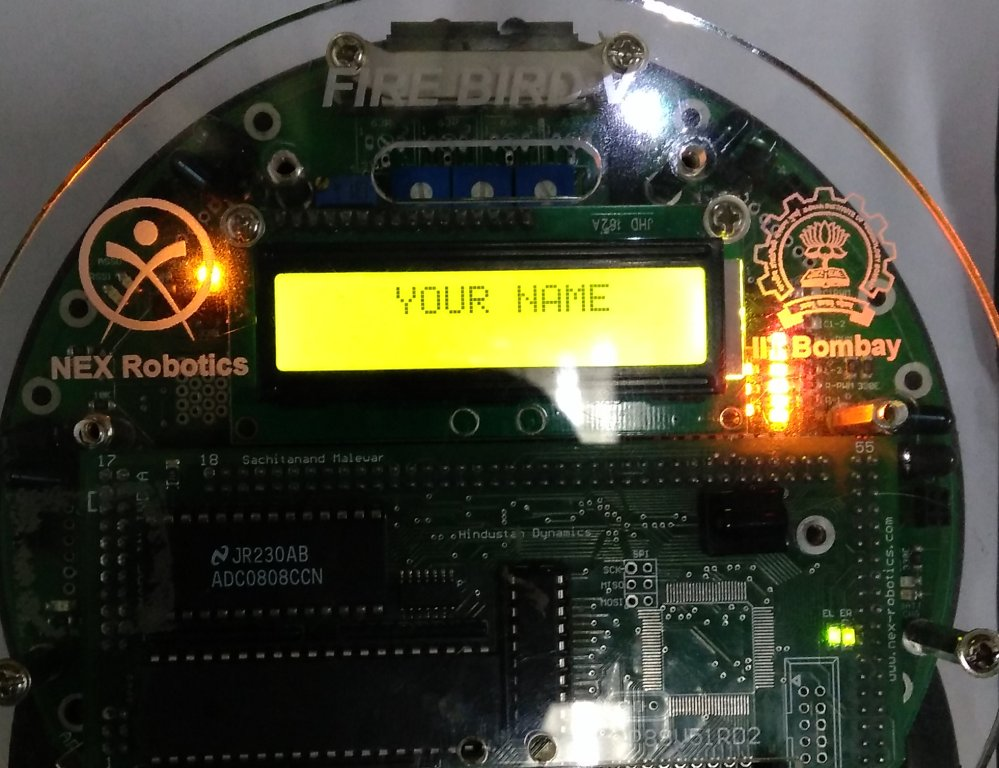
\includegraphics[scale=0.15]{lcd3.jpg}\\
					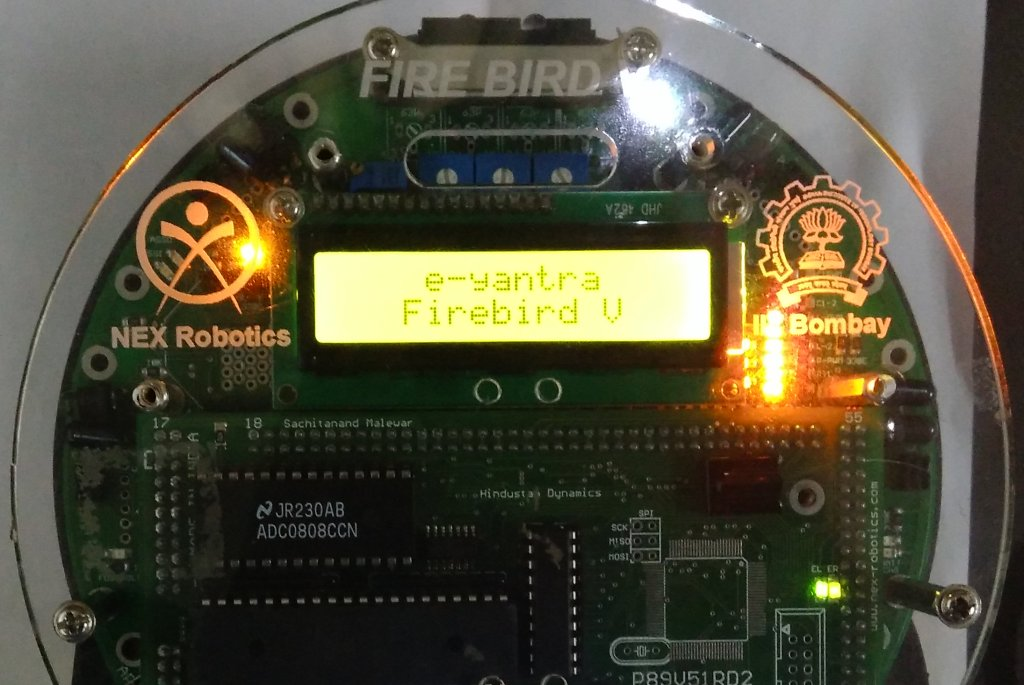
\includegraphics[scale=0.15]{lcd2.jpg}\\ \vspace{0.5cm}
					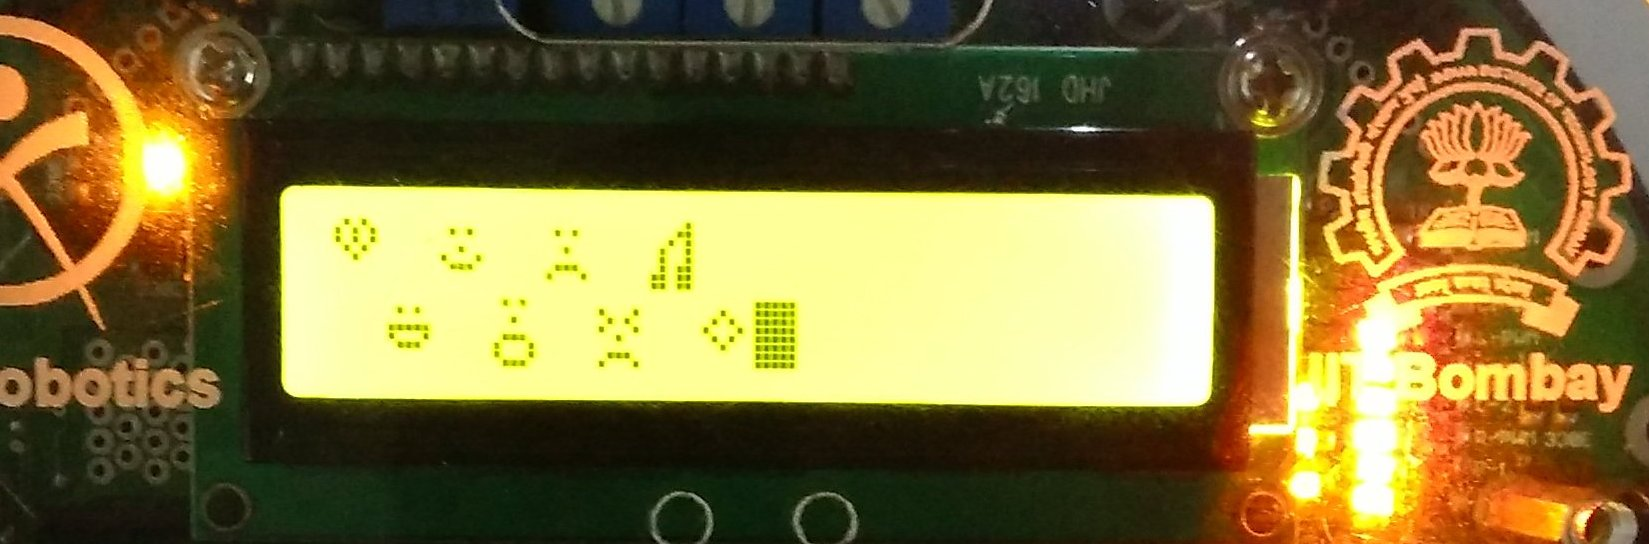
\includegraphics[scale=0.15]{lcd1.jpg}	\\
			\end{figure}
			\framebreak 
			\item Interrupts
			\begin{itemize}
				\item[$\checkmark$]External interrupt
				\item[$\checkmark$]Timer overflow interrupt
				\item[$\checkmark$]Serial interrupt
				\vspace{0.4cm}
			\end{itemize}
		
			\item Position encoders (use of external interrupt)\vspace{0.4cm}
			
			
			\item USB to serial communication
			\begin{itemize}
				
				\item[$\checkmark$]Loading Hex file into firebird V				   
				\item[$\checkmark$]USB to serial communication(using USB)				
			\end{itemize}
			\vspace{0.4cm}
		    \item Wireless communication using zigbee
		    \framebreak
			\item Interfacing Motors \newline
			\item PWM technique \newline
			\item Interfacing ADC \newline
			\item Interfacing White line sensors \newline
			\item Interfacing Sharp GP2D12C Infrared range sensor \newline
			\item Interfacing IR Proximity sensors \newline
			\item Battery voltage sensing \newline
		\end{enumerate}
		\item All the tasks are completed within the given deadlines.
		\framebreak
		\item Here is an idea for a small theme covering all concepts given above.
		\begin{itemize}
			\item[$\bullet$]\textbf{Theme name- }Automatic Car parking system
			\item[$\bullet$]\textbf{Description- }Robot will trace the arena and search for an empty slot, when it finds one it will automatically park itself.
		\begin{figure}[h]
				\includegraphics[scale=0.35]{arena.jpg}		
		\end{figure}
		\framebreak
			\item[$\bullet$]\textbf{Concepts covered } \newline
				\begin{enumerate}
					\item Line following \newline
					\item Obstacle detection and avoiding \newline
					\item LCD interfacing \newline
					\item Zigbee(serial interrupt) \newline
					\item Buzzer \newline
					\item Timer and External Interrupts \newline
				\end{enumerate}
				\framebreak
			\item Few more ideas for theme are \newline \newline
			 \begin{itemize}
			 	\item[$\bullet$]\textbf{Automatic newspaper distributor:}The robot will traverse the paths of a society and distribute correct newspapers and magazines to the required houses.\newline \newline
			 	\item[$\bullet$]\textbf{Farmhouse robot:}The robot will traverse the given path of a farmhouse and check if eggs are present at each node, if an egg is detected it will fetch it and send the message to the owner of farm.    
			 \end{itemize}
		\end{itemize}		 
	\end{itemize}
\end{frame}

\section{Challenges Faced}
\begin{frame}{Challenges Faced}
	\begin{itemize}
		\item Interfacing LED or any other IO device was a challenge as there is no expansion slot available.
		 \newline
		\item Because of the difference in speed of DC motors, motors based experiments seemed difficult.
		 \newline
		\item As P89V51RD2 supports only 3 proximity sensors that too in the front part so we were not able to make a perfect wall follower.
	\end{itemize}
\end{frame}

\section{Future Plans}
\begin{frame}{Future Plans}
	\begin{itemize}
		\item Designing a small theme covering all the concepts of 8051.\newline
		\item Learn ARM7 based Fire Bird V Robot. \newline
		\item Preparing the experiments for ARM7 based Fire Bird V Robot on the given modules. \newline
		\item Designing a small theme covering all the concepts of ARM7.\newline
		\item Making report, documentation and video tutorial of each module. \newline
	\end{itemize}
\end{frame}

\section{Thank You}
\begin{frame}{Thank You}
	\centering THANK YOU !!!
\end{frame}
\end{document}
